\documentclass[english,man]{apa6}

\usepackage{amssymb,amsmath}
\usepackage{ifxetex,ifluatex}
\usepackage{fixltx2e} % provides \textsubscript
\ifnum 0\ifxetex 1\fi\ifluatex 1\fi=0 % if pdftex
  \usepackage[T1]{fontenc}
  \usepackage[utf8]{inputenc}
\else % if luatex or xelatex
  \ifxetex
    \usepackage{mathspec}
    \usepackage{xltxtra,xunicode}
  \else
    \usepackage{fontspec}
  \fi
  \defaultfontfeatures{Mapping=tex-text,Scale=MatchLowercase}
  \newcommand{\euro}{€}
\fi
% use upquote if available, for straight quotes in verbatim environments
\IfFileExists{upquote.sty}{\usepackage{upquote}}{}
% use microtype if available
\IfFileExists{microtype.sty}{\usepackage{microtype}}{}

% Table formatting
\usepackage{longtable, booktabs}
\usepackage{lscape}
% \usepackage[counterclockwise]{rotating}   % Landscape page setup for large tables
\usepackage{multirow}		% Table styling
\usepackage{tabularx}		% Control Column width
\usepackage[flushleft]{threeparttable}	% Allows for three part tables with a specified notes section
\usepackage{threeparttablex}            % Lets threeparttable work with longtable

% Create new environments so endfloat can handle them
\newenvironment{ltable}
  {\begin{landscape}\begin{center}\begin{threeparttable}}
  {\end{threeparttable}\end{center}\end{landscape}}

\newenvironment{lltable}
  {\begin{landscape}\begin{center}\begin{ThreePartTable}}
  {\end{ThreePartTable}\end{center}\end{landscape}}

\usepackage{ifthen} % Only add declarations when endfloat package is loaded
\ifthenelse{\equal{\string man}{\string man}}{%
 \DeclareDelayedFloatFlavor{ThreePartTable}{table} % Make endfloat play with longtable
 \DeclareDelayedFloatFlavor{ltable}{table} % Make endfloat play with lscape
 \DeclareDelayedFloatFlavor{lltable}{table} % Make endfloat play with lscape & longtable
}{}%


% The following enables adjusting longtable caption width to table width
% Solution found at http://golatex.de/longtable-mit-caption-so-breit-wie-die-tabelle-t15767.html
\makeatletter
\newcommand\LastLTentrywidth{1em}
\newlength\longtablewidth
\setlength{\longtablewidth}{1in}
\newcommand\getlongtablewidth{%
 \begingroup
  \ifcsname LT@\roman{LT@tables}\endcsname
  \global\longtablewidth=0pt
  \renewcommand\LT@entry[2]{\global\advance\longtablewidth by ##2\relax\gdef\LastLTentrywidth{##2}}%
  \@nameuse{LT@\roman{LT@tables}}%
  \fi
\endgroup}


  \usepackage{graphicx}
  \makeatletter
  \def\maxwidth{\ifdim\Gin@nat@width>\linewidth\linewidth\else\Gin@nat@width\fi}
  \def\maxheight{\ifdim\Gin@nat@height>\textheight\textheight\else\Gin@nat@height\fi}
  \makeatother
  % Scale images if necessary, so that they will not overflow the page
  % margins by default, and it is still possible to overwrite the defaults
  % using explicit options in \includegraphics[width, height, ...]{}
  \setkeys{Gin}{width=\maxwidth,height=\maxheight,keepaspectratio}
\ifxetex
  \usepackage[setpagesize=false, % page size defined by xetex
              unicode=false, % unicode breaks when used with xetex
              xetex]{hyperref}
\else
  \usepackage[unicode=true]{hyperref}
\fi
\hypersetup{breaklinks=true,
            pdfauthor={},
            pdftitle={Why do we hate hypocrites?},
            colorlinks=true,
            citecolor=blue,
            urlcolor=blue,
            linkcolor=black,
            pdfborder={0 0 0}}
\urlstyle{same}  % don't use monospace font for urls

\setlength{\parindent}{0pt}
%\setlength{\parskip}{0pt plus 0pt minus 0pt}

\setlength{\emergencystretch}{3em}  % prevent overfull lines

\ifxetex
  \usepackage{polyglossia}
  \setmainlanguage{}
\else
  \usepackage[english]{babel}
\fi

% Manuscript styling
\captionsetup{font=singlespacing,justification=justified}
\usepackage{csquotes}
\usepackage{upgreek}



\usepackage{tikz} % Variable definition to generate author note

% fix for \tightlist problem in pandoc 1.14
\providecommand{\tightlist}{%
  \setlength{\itemsep}{0pt}\setlength{\parskip}{0pt}}

% Essential manuscript parts
  \title{Why do we hate hypocrites?}

  \shorttitle{Hypocrites}


  \author{First Author\textsuperscript{1}~\& Ernst-August Doelle\textsuperscript{1,2}}

  \def\affdep{{"", ""}}%
  \def\affcity{{"", ""}}%

  \affiliation{
    \vspace{0.5cm}
          \textsuperscript{1} Wilhelm-Wundt-University\\
          \textsuperscript{2} Konstanz Business School  }

  \authornote{
    \newcounter{author}
    Complete departmental affiliations for each author (note the
    indentation, if you start a new paragraph). Enter author note here.

                      Correspondence concerning this article should be addressed to First Author, Postal address. E-mail: \href{mailto:my@email.com}{\nolinkurl{my@email.com}}
                          }


  \abstract{Why do people judge hypocrites, who condemn immoral behaviors that they
in fact engage in, so negatively? We propose that hypocrites are
disliked because their condemnation sends a false signal about their
personal conduct, deceptively suggesting that they behave morally. We
show that verbal condemnation signals moral goodness (Study 1) and does
so even more convincingly than directly stating that one behaves morally
(Study 2). We then demonstrate that people judge hypocrites
negatively---even more negatively than people who directly make false
statements about their morality (Study 3). Finally, we show that
``honest'' hypocrites---who avoid false signaling by admitting to
committing the condemned transgression---are not perceived negatively
even though their actions contradict their stated values (Study 4).
Critically, the same is not true of hypocrites who engage in false
signaling but admit to unrelated transgressions (Study 5). Together, our
results support a false-signaling theory of hypocrisy}
  \keywords{moral psychology, condemnation, vignettes, deception, social signaling,
open data, open materials \\

    \indent Word count: X
  }





\usepackage{amsthm}
\newtheorem{theorem}{Theorem}
\newtheorem{lemma}{Lemma}
\theoremstyle{definition}
\newtheorem{definition}{Definition}
\newtheorem{corollary}{Corollary}
\newtheorem{proposition}{Proposition}
\theoremstyle{definition}
\newtheorem{example}{Example}
\theoremstyle{remark}
\newtheorem*{remark}{Remark}
\begin{document}

\maketitle

\setcounter{secnumdepth}{0}



Consider the hypocrite---someone who condemns the moral failings of
other people but behaves badly him- or herself. Many commentators have
remarked on the \enquote{peculiarly repulsive} nature of hypocrisy
(Shklar, 1984, p. 57). The degree to which hypocrites are disliked
cannot be explained by their transgressions alone: What makes hypocrites
especially bad is that they both commit a transgression and condemn it.
But why is this combination so objectionable? After all, speaking out
against immorality is normally seen as laudable. It enforces norms and
encourages moral behavior (Berkowitz \& Walker, 1967; Feinberg, Willer,
\& Schultz, 2014; Feinberg, Willer, Stellar, \& Keltner, 2012), such
that failing to condemn transgressions has been characterized as
secondorder free-riding (Yamagishi, 1986). Arguably, then, people should
not be so resentful toward hypocrites: They may fail to achieve their
moral aspirations, but at least they oppose bad behavior

\section{Method}\label{method}

\subsection{Design}\label{design}

To test these predictions, we presented subjects with vignettes and
asked them to evaluate target characters in the vignettes. In a 2 × 2
between-subjects design, we manipulated whether the targets engaged in
moral condemnation or not and whether subjects had direct information
about the targets' moral behavior or not. We predicted that subjects
would evaluate targets who engaged in moral condemnation more positively
than those who did not, but only in the absence of direct information
about the targets' moral behavior.

\subsection{Participants}\label{participants}

Study 1 contained 619 participants.

\subsection{Materials}\label{materials}

\subsection{Procedure}\label{procedure}

In each of our vignettes, we asked subjects to imagine that they
belonged to a social group in which a particular moral transgression was
possible (e.g., a track team whose members might use forbidden
performance-enhancing drugs). Subjects were then told about two members
of the social group: the target (whom subjects would later evaluate) and
the other person (whom subjects would not evaluate), both of whom were
described neutrally (not using these terms).

\subsection{Data analysis}\label{data-analysis}

We used R (3.3.2, R Core Team, 2016) and the R-packages
\emph{BayesFactor} (0.9.12.2, Morey \& Rouder, 2015), \emph{coda}
(0.19.1, Plummer, Best, Cowles, \& Vines, 2006), \emph{dplyr} (0.5.0,
Wickham \& Francois, 2016), \emph{jpeg} (0.1.8, Urbanek, 2014),
\emph{Matrix} (1.2.8, Bates \& Maechler, 2017), \emph{papaja}
(0.1.0.9456, Aust \& Barth, 2016), \emph{rprojroot} (1.2, Müller, 2017),
and \emph{yarrr} (0.1.4, Phillips, 2017) for all our analyses. Raw data
are available at the Open Science Framework at
\url{https://osf.io/pszjz/}

\section{Results}\label{results}

To test our predictions, we conducted a 2 (condemnation condition:
target condemns vs.~other condemns) × 2 (information condition: good
information vs.~no information) analysis of variance (ANOVA) predicting
mean positive evaluations of the targets across the vignettes (see
Figure \ref{fig:figure1}). We found a significant main effect of
information condition \(F(1, 615) = 136.43\), \(\mathit{MSE} = 0.64\),
\(p < .001\), \(\eta^2_G = .182\). subjects evaluated targets more
positively in the good-information condition (M = 5.28, sd = 0.83), than
in the no-information condition (M = 4.52, sd = 0.8). This result served
as a manipulation check, demonstrating that direct positive information
about the target's moral behavior was perceived as a clear indication of
moral goodness.

We also found a significant main effect of condemnation condition,
\(F(1, 615) = 12.79\), \(\mathit{MSE} = 0.64\), \(p < .001\),
\(\eta^2_G = .020\) subjects evaluated targets more positively when the
target engaged in condemnation (M = 5.01, sd = 0.91) than when the other
person engaged in condemnation (M = 4.81, sd = 0.87). This result
confirmed our hypothesis that moral condemnation serves as a signal of
moral goodness.

Finally, we found a significant interaction, \(F(1, 615) = 8.51\),
\(\mathit{MSE} = 0.64\), \(p = .004\), \(\eta^2_G = .014\); the target's
use of condemnationhad a larger effect in the no-information condition
than in the good-information condition. Specifically, when subjects were
given no information about the target's behavior, they evaluated the
target significantly more positively when he or she condemned the
transgression (M = 4.73, sd = 0.94) than when the other party condemned
the transgression (M = 4.31, sd = 0.55), \(\Delta M = 0.42\), 95\% CI
\([-0.60\), \(-0.25]\), \(t(249.22) = -4.81\), \(p < .001\).

However, in the good-information condition, we found no significant
difference between the target-condemns condition (M = 5.3, sd = 0.79)
and the other-condemns condition (M = 5.25, sd = 0.87),
\(\Delta M = 0.05\), 95\% CI \([-0.23\), \(0.14]\),
\(t(313.96) = -0.50\), \(p = .620\)

This result confirmed our hypothesis that observers rely on a person's
statements of condemnation as a signal of moral goodness only when they
lack direct information about the person's moral behavior.

We note that the null effect of the target expressing condemnation in
the good-information condition does not appear to be a ceiling effect.
In the good-information condition, the mean composite evaluation (5.28)
was substantially below the scale's ceiling (7), and subjects rarely
used the ceiling value (only 6\% of responses to the evaluative
questions were a \enquote{7})

\begin{figure}[htbp]
\centering
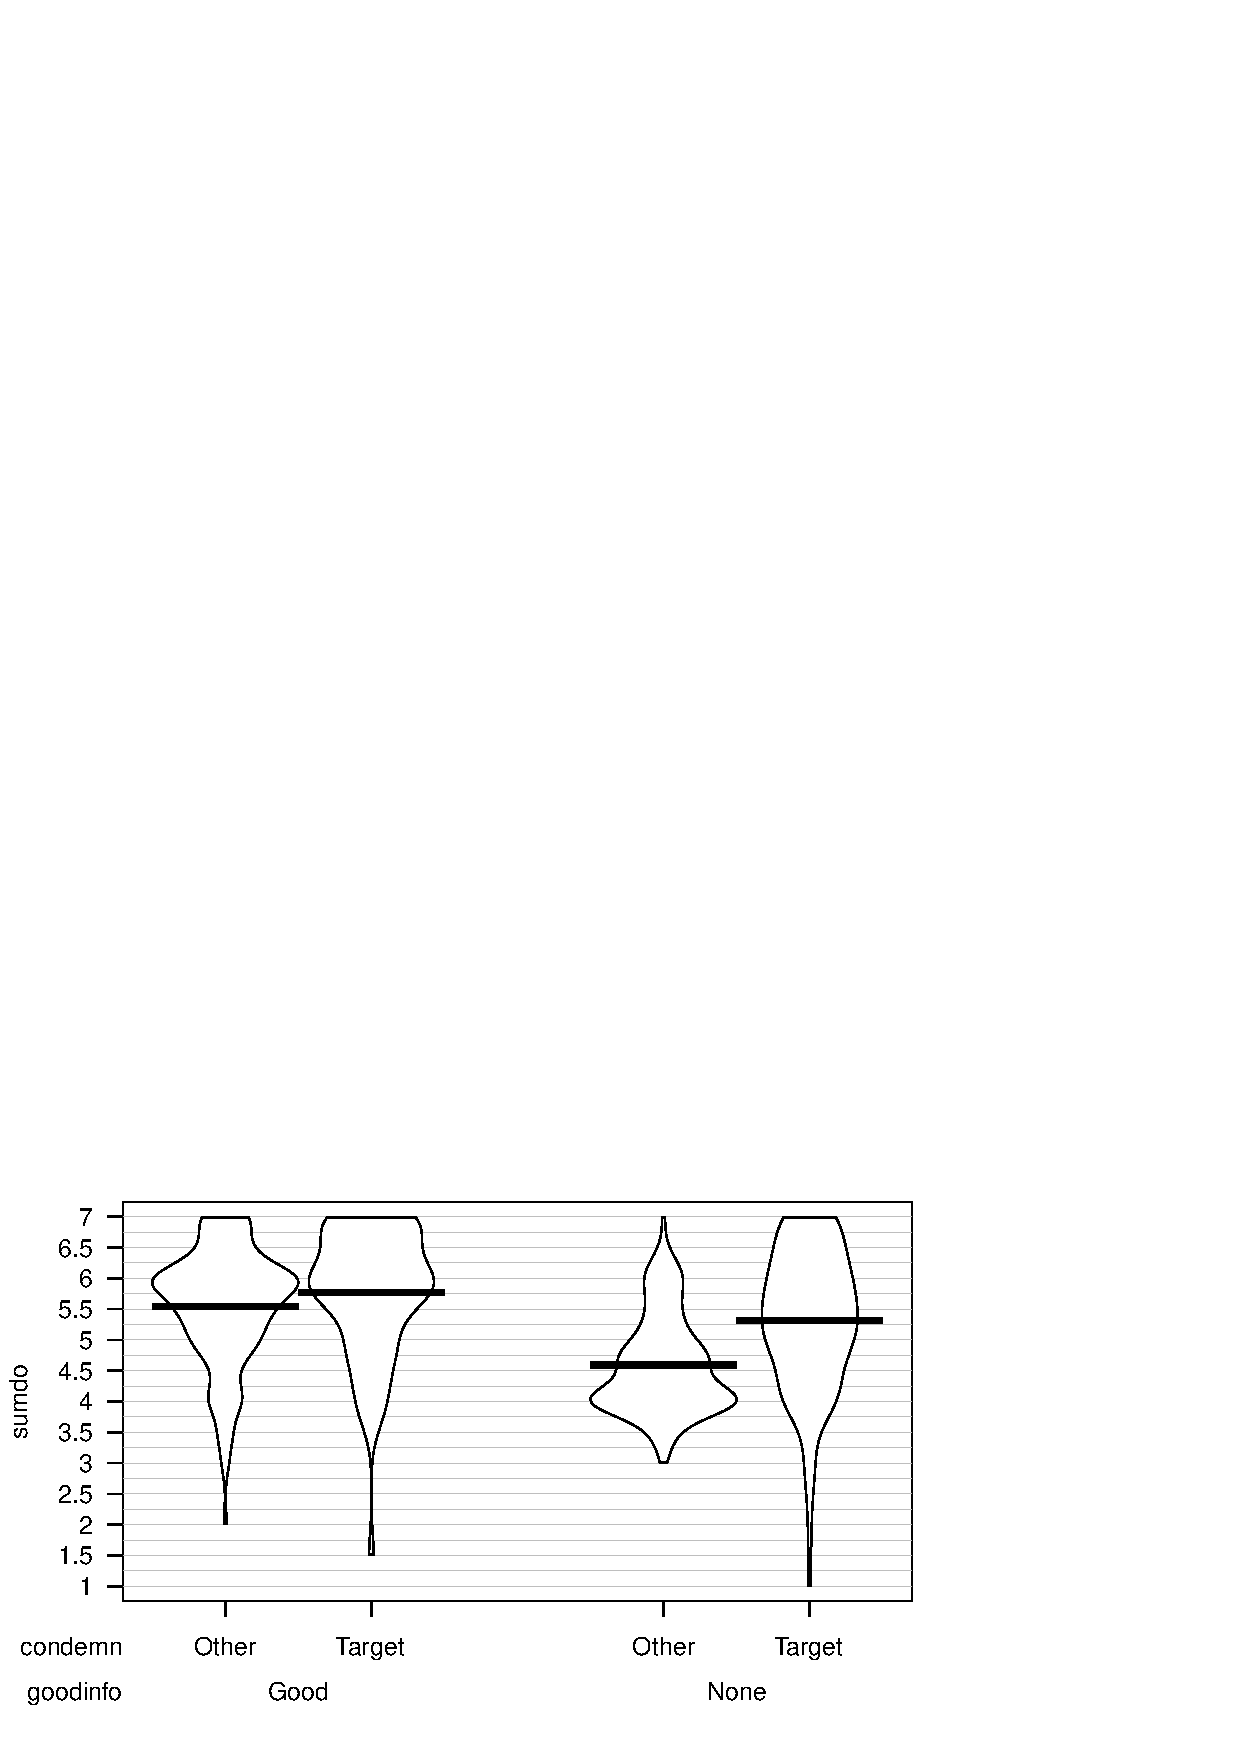
\includegraphics{jordan_apa_files/figure-latex/figure1-1.pdf}
\caption{\label{fig:figure1}Results from Study 1: mean composite evaluation
of the targets as a function of condemnation condition and information
condition. Error bars represent 95\% Bayesian highest density
intervals.}
\end{figure}

\section{Discussion}\label{discussion}

Really great discussion

\newpage

\section{References}\label{references}

\setlength{\parindent}{-0.5in} \setlength{\leftskip}{0.5in}

\hypertarget{refs}{}
\hypertarget{ref-R-papaja}{}
Aust, F., \& Barth, M. (2016). \emph{Papaja: Create apa manuscripts with
rmarkdown}. Retrieved from \url{https://github.com/crsh/papaja}

\hypertarget{ref-R-Matrix}{}
Bates, D., \& Maechler, M. (2017). \emph{Matrix: Sparse and dense matrix
classes and methods}. Retrieved from
\url{https://CRAN.R-project.org/package=Matrix}

\hypertarget{ref-berkowitz1967laws}{}
Berkowitz, L., \& Walker, N. (1967). Laws and moral judgments.
\emph{Sociometry}, 410--422.

\hypertarget{ref-feinberg2014gossip}{}
Feinberg, M., Willer, R., \& Schultz, M. (2014). Gossip and ostracism
promote cooperation in groups. \emph{Psychological Science},
\emph{25}(3), 656--664.

\hypertarget{ref-feinberg2012virtues}{}
Feinberg, M., Willer, R., Stellar, J., \& Keltner, D. (2012). The
virtues of gossip: Reputational information sharing as prosocial
behavior. \emph{Journal of Personality and Social Psychology},
\emph{102}(5), 1015.

\hypertarget{ref-R-BayesFactor}{}
Morey, R. D., \& Rouder, J. N. (2015). \emph{BayesFactor: Computation of
bayes factors for common designs}. Retrieved from
\url{https://CRAN.R-project.org/package=BayesFactor}

\hypertarget{ref-R-rprojroot}{}
Müller, K. (2017). \emph{Rprojroot: Finding files in project
subdirectories}. Retrieved from
\url{https://CRAN.R-project.org/package=rprojroot}

\hypertarget{ref-R-yarrr}{}
Phillips, N. (2017). \emph{Yarrr: A companion to the e-book ``yarrr!:
The pirate's guide to r''}. Retrieved from
\url{https://CRAN.R-project.org/package=yarrr}

\hypertarget{ref-R-coda}{}
Plummer, M., Best, N., Cowles, K., \& Vines, K. (2006). CODA:
Convergence diagnosis and output analysis for mcmc. \emph{R News},
\emph{6}(1), 7--11. Retrieved from
\url{https://journal.r-project.org/archive/}

\hypertarget{ref-R-base}{}
R Core Team. (2016). \emph{R: A language and environment for statistical
computing}. Vienna, Austria: R Foundation for Statistical Computing.
Retrieved from \url{https://www.R-project.org/}

\hypertarget{ref-shklar1984ordinary}{}
Shklar, J. N. (1984). \emph{Ordinary vices}. Harvard University Press.

\hypertarget{ref-R-jpeg}{}
Urbanek, S. (2014). \emph{Jpeg: Read and write jpeg images}. Retrieved
from \url{https://CRAN.R-project.org/package=jpeg}

\hypertarget{ref-R-dplyr}{}
Wickham, H., \& Francois, R. (2016). \emph{Dplyr: A grammar of data
manipulation}. Retrieved from
\url{https://CRAN.R-project.org/package=dplyr}






\end{document}
